
\section{Inconic and Circumconic of a triangle}
\label{app:A-inconic}

Two triangles $T=ABC$ and $T_1=A_1B_1C_1$ are called in perspective when  the three lines $AA_1$, $BB_1$ and $CC_1$ are concurrent. This point is called the perspector of the pair $\{T,T_1\}$.

Also, the perspective axis of a pair of triangles is the line passing through the   three points of intersection of the correspondent sidelines $AB\cap A_1B_1$,
$AC\cap A_1C_1$ and $BC\cap B_1C_1$.
See \cref{fig:appA-perspector}.
\begin{figure}
    \centering
    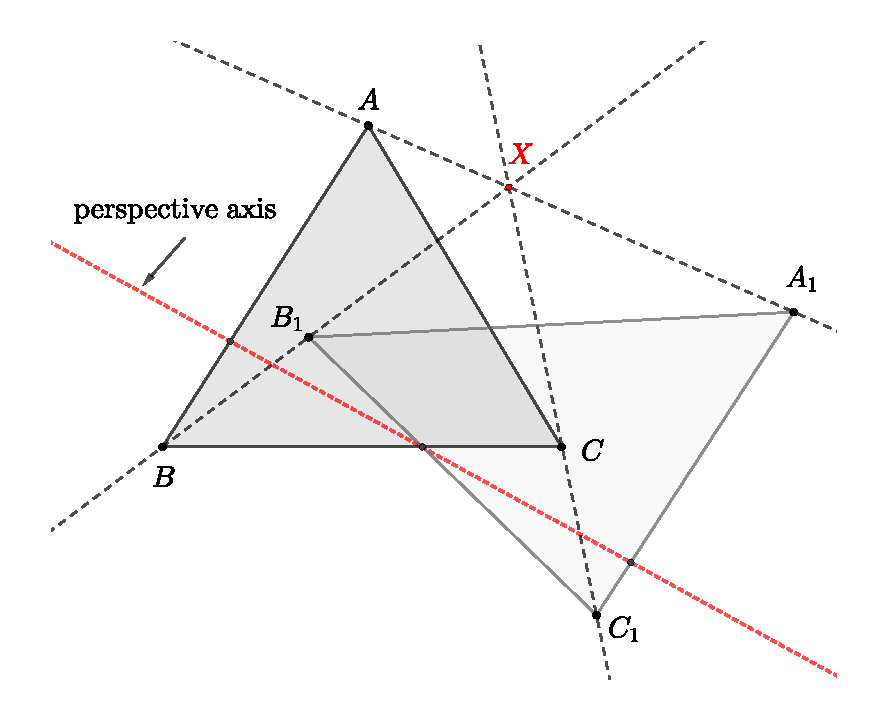
\includegraphics[scale=0.4]{zappA/pics/pics-appA-101-perspector.pdf}
    \caption{Perspector and perspective axis of a pair of triangles $ABC$ and $A_1B_1C_1$.}
    \label{fig:appA-perspector}
\end{figure}

Given a triangle $T=ABC$ and a conic $\E$ the polar triangle of $T$ with respect to $\E$ is the triangle whose sidelines are the polar lines of the vertices   $A,B,C$. See \cref{fig:appA-polar-triangle}
\begin{figure}
    \centering
    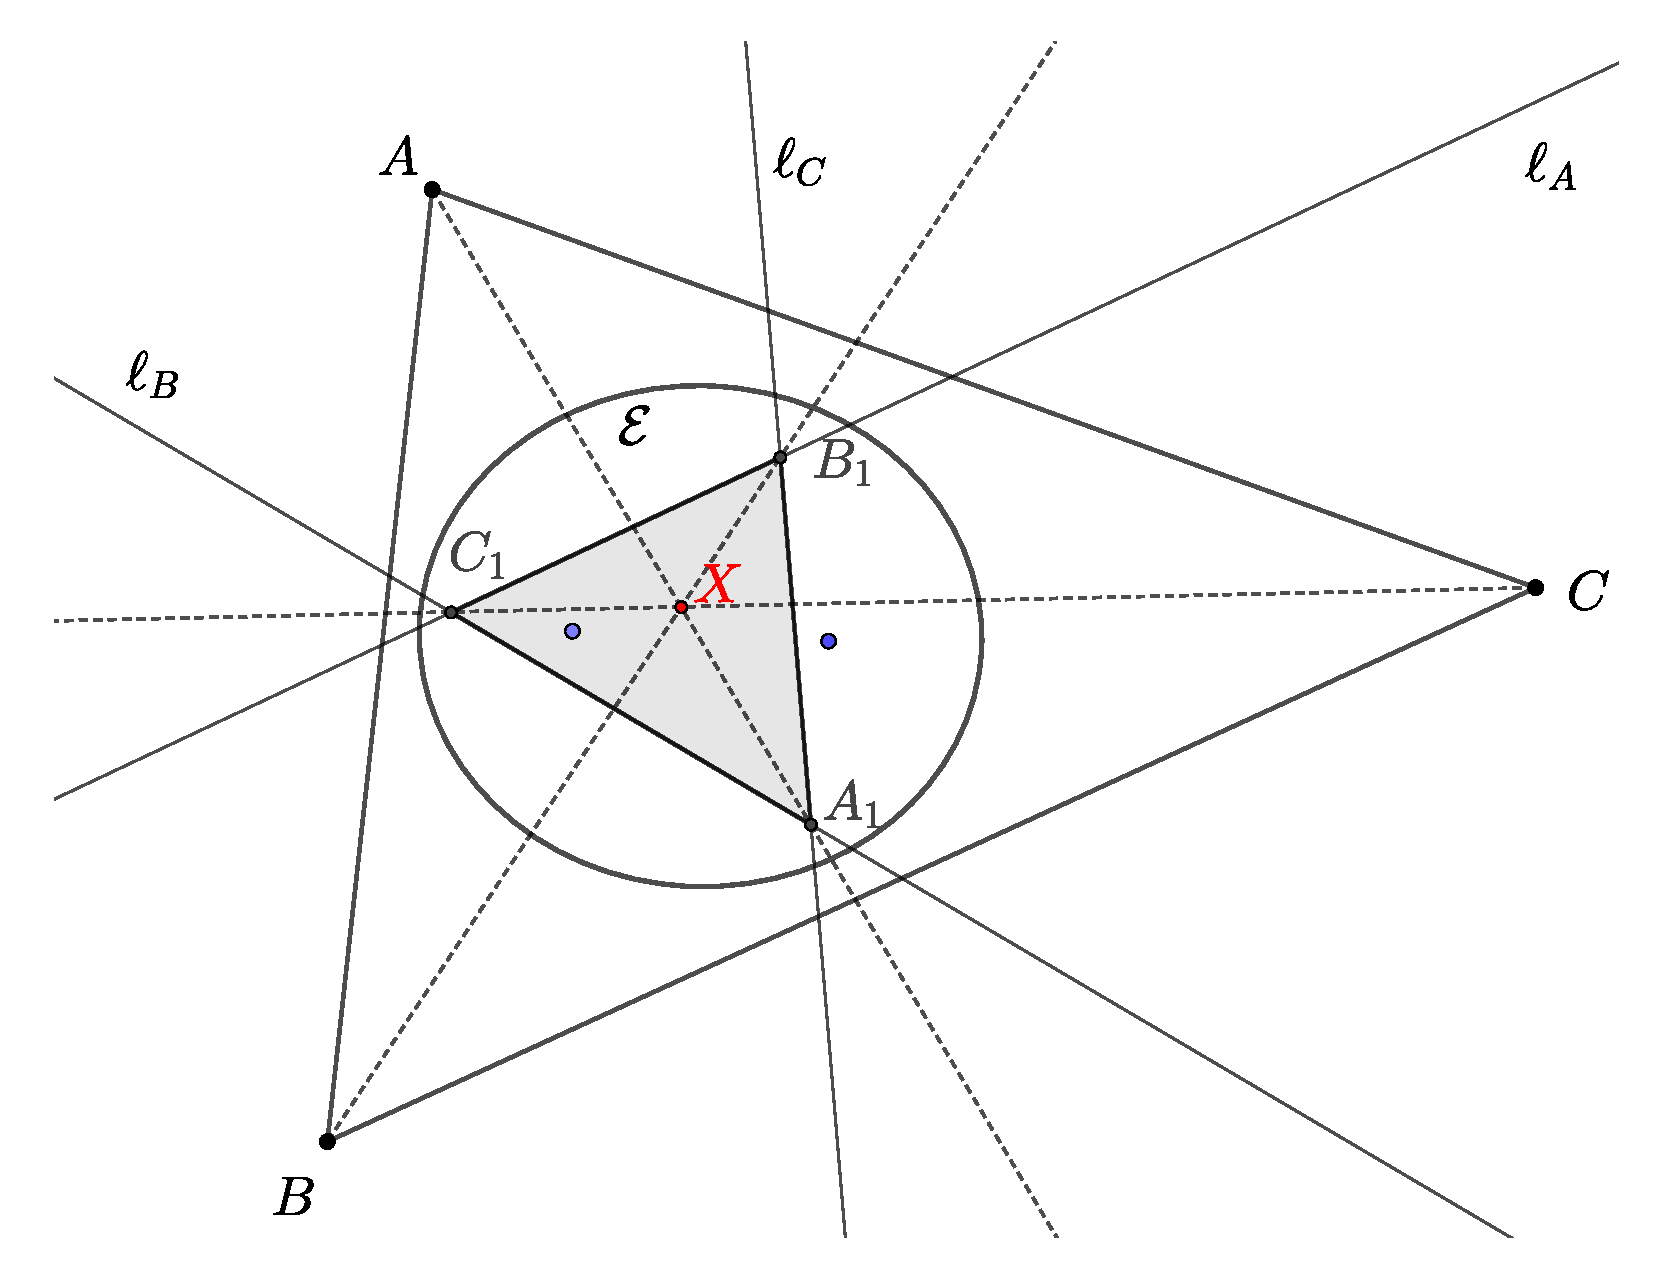
\includegraphics[scale=0.3]{zappA/pics/pics-appA-150-perspector-triangle-ellipse.pdf}
    \caption{Polar triangle $A_1B_1C_1$ and perspector $X$.}
    \label{fig:appA-polar-triangle}
\end{figure}

A conic $\E$ that is tangent to the sidelines of a triangle $ABC$ is called {\em inconic}. The perspector of the triangles $ABC$ and its polar with respect to $\E$ is called the perspector of the inconic.

In   an elliptic  billiard having a 3-periodic orbit, i.e., a triangle $T=ABC$ the perspector of the caustic is the triangular center $X_8$ of $T$. The perspector of the billiard is $X_1$. See \cref{fig:appA-X8-X1-perspectors}.
\begin{figure}
    \centering
    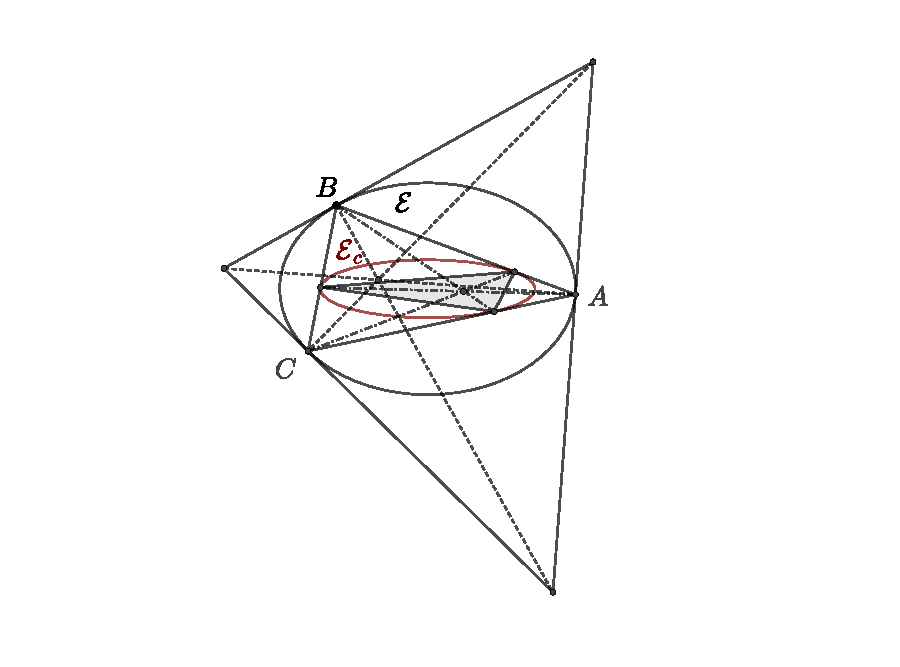
\includegraphics[scale=0.7]{zappA/pics/pics-appA-170-inconic-billiardggb.pdf}
    \caption{Perspectors of the caustic $\E_c$ is $X_8$ o and of the billiard $\E$ is the $X_1$ (incenter). }
    \label{fig:appA-X8-X1-perspectors}
\end{figure}

Given a triangle $T=ABC$ the conic passing through the vertices is called {\em circumconic}. The circumconic is unique when the center is fixed; otherwise we have a 2d-family of circumconics circumscribing a given triangle. 



	\section{Isogonal and isotomic conjugation}
	
	Consider a triangle $T=ABC$ and a point $P$. Denote by $A_1$, $B_1$ and $C_1$ the contact points of the sidelines of $T$ with the incircle. Consider the reflection of the line $AP$ with respect to $AA_1$ and repeat this process for the other two lines, i.e., reflect the line $BP$ (resp. $PC$) with respect to the bisector $BB_1$ (resp. $CC_1$).
	The intersection of these three reflected lines is called the {\em isogonal conjugate} of $P$. 
	
	Analogously, when we consider reflection of points  with respect to midpoints   we obtain the so called {\em isotomic conjugate} of $P$. More precisely, consider the intersection $A_1$ of the line $AP$ with the sideline $BC$. Reflect $A_1$ with respect to the midpoint $A_m$ of the side $BC$ obtaining the point $A_1'$. Repeat for the other two sides obtaining the points $B_1'$ and $C_1'$. The intersection of the three lines $AA_1'$, $BB_1'$ and $CC_1'$ is the isotomic conjugate of $P$.
	
		\begin{figure}
	    \centering
	    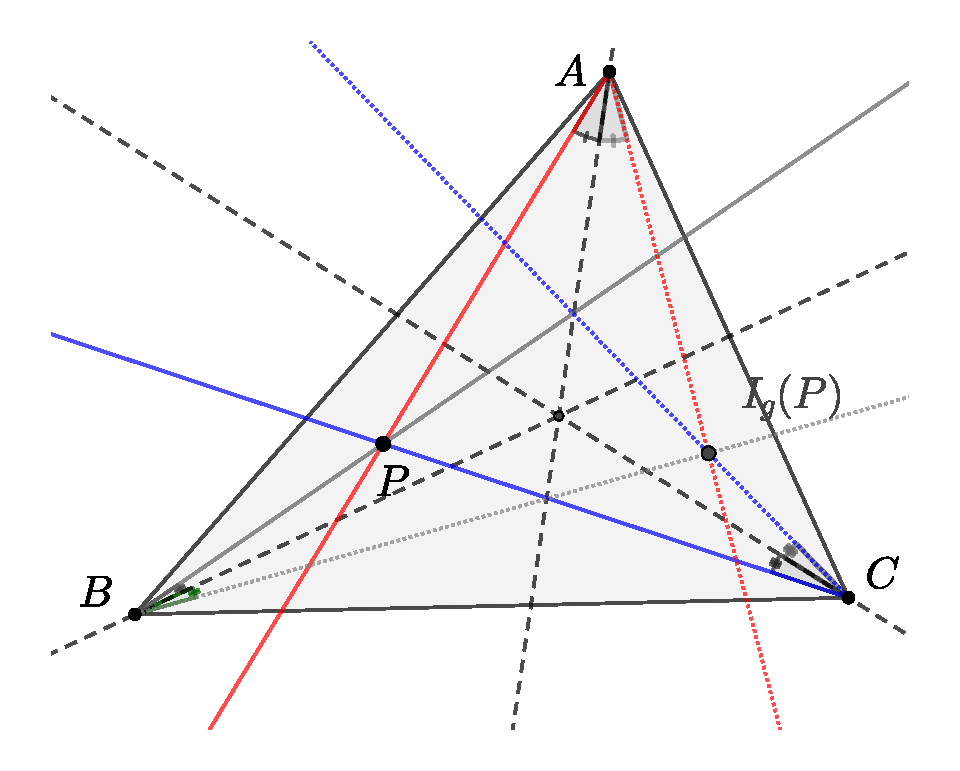
\includegraphics[scale=0.35]{zappA/pics/pics-appA_180-isogonal.pdf}
	     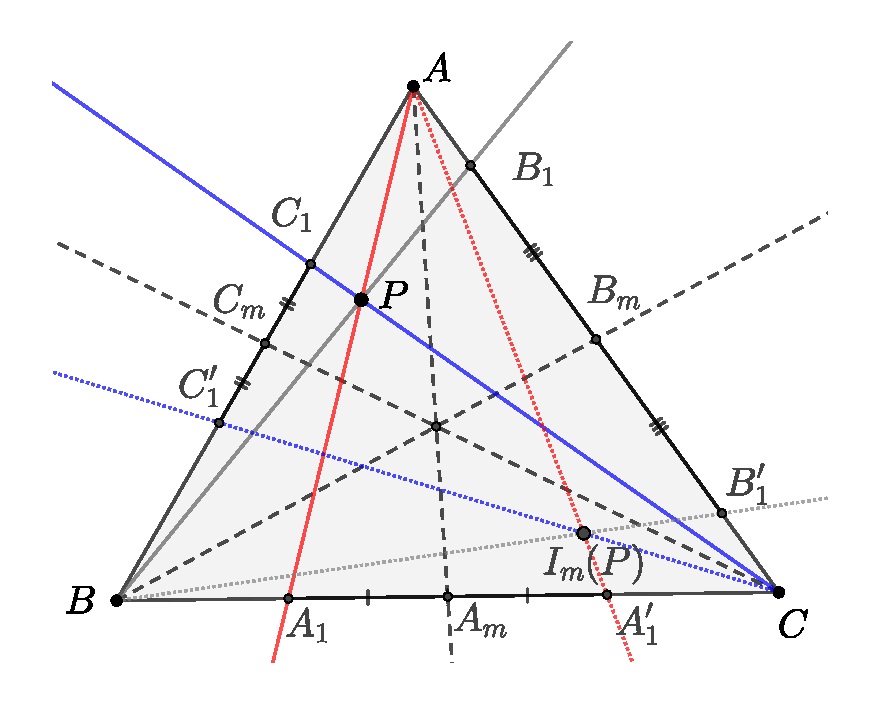
\includegraphics[scale=0.4]{zappA/pics/pics-appA_190-isotomic.pdf}
	    \caption{Isogonal and isotomic conjugatation.}
	    \label{fig:appA-isotomic-isogonal}
	\end{figure}

	 \begin{remark}
 The concept of reflection used here is that of projective geometry. This means that the cross-ratio of the four aligned points, say $A=( a,0,1)$, $B=(b,0,1)$, $C=(c,0,1)$ and $D=(d,0,1)$ is given by:
 \[ [A,B,C,D]=\frac{(c-a)(d-b)}{(d-a)(c-b)}\]
 \end{remark}
	\begin{proposition}
	Let $P=[p,q,r]$ given in trilinear coordinates. Then the isogonal conjugate of $P$ is $[1/p,1/q,1/r]$.
	\end{proposition}
	
	\begin{proof} In trilinear coordinates. Let $P=[p,q,r]$, $A=[1,0,0]$, $B=[0,1,0] $ and $C=[0,0,1]$.
	Then $A_1=[0,1,1]$, $B_1=[1,0,1]$ and $C_1=[1,0,0]$. The line $AP$ is given by
	$q z - r y=0$ and their reflection in relation to the bisector $z=y$ is the line $  q y-r z=0$. Analogously, the other two reflected lines are given by $ x p-r z=0$ and $p x-q y=0$. The intersection of these three lines is 
	\[ [\frac{r z}{p},\frac{r z}{q},\frac{r z}{r}]= [\frac{1}{p},\frac{1}{q},\frac{1}{r}]\]
	\end{proof}

	 
	
		\begin{proposition}
	Let $P=[p,q,r]$ given in trilinear coordinates. Then the isotomic  conjugate of $P$ is $[1/(a^2 p),1/(b^2 q),1/(c^2 r)]$.
	When $P=[p,q,r]_b$ is given in barycentric coordinates   the isotomic conjugate of $P$ is simply $[1/p, 1/q, 1/r]_b$.
	\end{proposition}
 \begin{proof}
 In trilinear coordinates,  let $P=[p,q,r]$, $A=[1,0,0]$, $B=[0,1,0] $ and $C=[0,0,1]$.
	Then the midpoint of the side $BC$ is $A_m=[0,c,b]$. Also, $B_m=[c,0,a]$ and $C_m=[b,a,0]$. The line $AP$ is given by
	$q z - r y=0$. Therefore $A_1=[0,q,r]$ and $A_1'=[0,c^2r,b^2q]$. 
 
	Analogously, the   line $BP$ is given by $   r x-p z=0  $. Therefore $B_1=[ p,0,r]$ and
	$B_1'=[r^ 2c,0,a^2p]$.  
	Therefore the intersection of the   lines $AA_1'$ and $BB_1'$ is the point
	\[[\frac{1}{  a^2 p},\frac{1}{b^2 q},\frac{1}{c^2 r} ] \]
 \end{proof}
 
	\begin{remark}
	Under isogonal conjugation it follows that
	\[\angle P A B = \angle C A I_g(P),\;\; \angle P B C = \angle A B I_g(P),\;\; \angle P C A = \angle B  C I_g(P)\]
	\end{remark}
	The isogonal conjugation is the map $I_g([p,q,r])=[1/p,1/q,1/r]=[q r,p r,p q]$ which is an involution $(I_g\circ I_g=id)$.
	
	The isomotic conjugation is the map $I_m([p,q,r])=[1/(a^2p),1/(b^2 q),1/(c^2r)]=[  q r/a^2, p r/b^2, p q/c^2]$ which is also an involution.

	\begin{proposition} The image of the Euler line by $I_g$ is the circumconic (hyperbola) given by
	
	\begin{align*}
\mathcal{I}_E(x,y,z)&=-c \left( a^2-b^2 \right)   \left( {a}^{2}+{b}^{2}-{c}^
{2} \right) x y+b \left( a^2-c^2 \right)    \left( {a}^{2
}-{b}^{2}+{c}^{2} \right) x z\\
&+a \left( b^2-c^2 \right)  
 \left( {a}^{2}-{b}^{2}-{c}^{2} \right) y z  =0
	\end{align*}
	More general, the image of any line by $I_g$ is a  circumconic.
	\end{proposition}
	
	\begin{proof} Write the Euler line in the parametric form $E(u)=(1-u)X_3+uX_4$ and compute $I_g(E(u))$. Now, writing in the implicit form, it is straightforward to obtain the result stated.
	\end{proof}
	
		\begin{proposition} The image of the Euler line by $I_m$ is circumconic (hyperbola)  by:
	
	\begin{align*}
\mathcal{I}_H(x,y,z)&= a b (a^2 - b^2) (a^2 + b^2 - c^2) x y - a c (a^2 - c^2) (a^2 - b^2 + c^2) x z \\
&- b c (b^2 - c^2) (a^2 - b^2 - c^2)y z=0
	\end{align*}
	
	\end{proposition}
	
	\begin{proof}
	Left to the reader.
	\end{proof}
	
	\begin{proposition} A   billiard  having a triangle $T=ABC$ as 3-periodic orbit is the isogonal conjugate of the antiorthic axis of $T$.
 \label{prop:appA-billiard-antiorthic}
	\end{proposition}
	\textcolor{red}{checar calculo da prova}
	\begin{proof}
	Recall that the antiorthic axis  is the perspective axis of the T and its excentral triangle, and that the elliptic billiard is centered at $X_9$ (mittenpunkt) and its perspector is   $X_1$ (incenter).
	Therefore, it follows that the antiorthic axis is given by $x+y+z=0$.
The elliptic billiard is $xy+xz+yz=0$.
	\end{proof}
	
%\textcolor{red}{ver que coordenada usa na observacao abaixo}
%	\begin{remark}
%	A circumconic with center $[x_0,y_0,z_0]$ is given by
%	\[(x_0-y_0-z_0) y z+(y_0-x_0-z_0) x z+ (z_0-x_0-y_0) xy=0\]
%	In the billiard the center is $X_9=[b + c - a , c + a - b , a + b - c]$.
%	
%	\end{remark}